\documentclass{article}
\usepackage{gvv}
\usepackage{gvv-book}
\begin{document}
\begin{center}
POLYNOMIAL
\end{center}
\begin{enumerate}
\item Let $P\left(x\right)$ be a non-zero polynomial with integer coefficients. If $P\left(n\right)$ is divisible by $n$ for each positive integer $n$, what is the value of $P\left(0\right)$ ?
\end{enumerate}

\begin{center}
QUADRATIC
\end{center}
\begin{enumerate}
\item The equations $x^2-4x+k=0$ and $x^2+kx-4=0$, where $k$ is a real number, have exactly one common root. What is the value of $k$ ?
\end{enumerate}


\begin{center}
SPEED TIME
\end{center}
\begin{enumerate}
\item A man walks a certain distance and rides back in $3\frac{3}{4}$ hours he could ride both ways in $2\frac{1}{2}$ hours. How many hours would it take him to walk both ways?
\end{enumerate}
\begin{center}
	\textbf ALGEBRA 
\end{center}
\begin{enumerate}
	\item Positive integers $a$ and $b$ are such that $a+b$ = $a/b+b/a$. What is the value of $a^2+b^2$ ? $[2]$
	\item At a party, each man danced with exactly four women and each woman danced with exactly
three men. Nine men attended the party. How many women attended the party? $[12]$
\item Let $a$, $b$ and $c$ be real numbers such that $a-7b+8c=4$ and $8a+4b-c=7$. What is the value of $a^2-b^2+c^2$? $[1]$
\item If $3^x+2^y=985$ and $3^x-2^y=473$. What is the value of $xy$? $[48]$
\item Let $n$ be the largest integer that is the product of exactly $3$ distinct prime numbers, $x$,$y$ and
$10x + y$, where $x$ and $y$ are digits. What is the sum of the digits of $n$? $[12]$
\item Let $a$, $b$ and $c$ be such that $a + b + c = 0$ and
	\begin{center}
		$P= \frac{a^2}{2a^2+bc} + \frac{b^2}{2b^2+ca} + \frac{c^2}{2c^2+ab}$
	\end{center}
		is defined. What is the value of $P$? $[1]$
\end{enumerate}

\begin{center}
GEOMETRY
\end{center}
\begin{enumerate}
\item How many line segments have both their endpoints located at the vertices of a given cube?
\item What is the greatest possible perimeter of a right-angled triangle with integer side lengths if one of the sides has length $12$?
\item A $2 \times 3$ rectangle and a $3 \times 4$ rectangle are contained within a square without overlapping at any interior point, and the sides of the square are parallel to the sides of the two given rectangles. What is the smallest possible area of the square?
\item In rectangle $ABCD$, $AB = 8$ and $BC = 20$. Let $P$ be a point on $AD$ such that $\angle BPC=90\degree$. If $r1$, $r2$, $r3$ are the radii of the incircles of triangles $APB$,$BPC$ and $CPD$, what is the value of $r1 + r2 + r3$?
\item A subset $B$ of the set of first $100$ positive integers has the property that no two elements of $B$ sum to $125$. What is the maximum possible number of elements in $B$?
\item In acute-angled triangle $ABC$, let $D$ be the foot of the altitude from $A$, and $E$ be the midpoint of $BC$. Let $F$ be the midpoint of $AC$. Suppose $\angle BAE = 40\degree$.If $\angle DAE = \angle DFE$, what is the magnitude of $\angle ADF$ in degrees?
\item The figure below shows a broken piece of a circular plate made of glass.
	\begin{figure}[h]
		\centering
		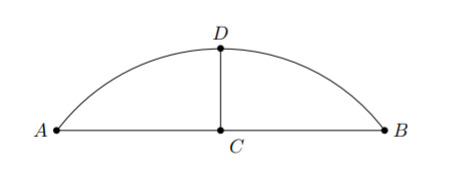
\includegraphics[width=\columnwidth]{finallatex.jpg}
	\end{figure}
$C$ is the midpoint of $AB$, and $D$ is the midpoint of arc $AB$. Given that $AB = 24 cm$ and $CD = 6 cm$, what is the radius of the plate in centimetres? $\left(The figure is not drawn to scale.\right)$
\end{enumerate}

\begin{center}
NUMBER THEORY
\end{center}
\begin{enumerate}
\item How many two-digit positive integers $N$ have the property that the sum of $N$ and the number obtained by reversing the order of the digits of $N$ is a perfect square?
\item Let $E\left(n\right)$ denote the sum of the even digits of $n$. For example, $E\left(1243\right) = 2 + 4 = 6$. What is the value of $E\left(1\right) + E\left(2\right) + E\left(3\right)+ \dots + E\left(100\right)$ ?
\item The digits of a positive integer $n$ are four consecutive integers in decreasing order when read from left to right. What is the sum of the possible remainders when $n$ is divided by $37$ ? 
\end{enumerate}
\end{document}
